\documentclass[english,11pt,a4paper,titlepage]{article}

\usepackage{fontspec} % !!!Requires compiling with either XeLaTeX or LuaLaTeX!!! - allows for advanced font selection - also handles font encoding. If you wish to use PDFLaTeX with a natively supported font, you can use the following package instead:
% \usepackage[T1]{fontenc} 

\usepackage{amsmath} % Package for math notation
\usepackage{fontspec} % Requires either XeLaTeX or LuaLaTeX
\usepackage{titlesec} % Allows alternative section titles
\usepackage{lastpage} % Used for "n of m" page numbering
\usepackage{afterpage} % Used to remove background color from pages after title page
\usepackage{amsmath} % Package for math notation
\usepackage{setspace}% Package for easy line spacing 
\usepackage{titlesec} % Allows alternative section titles
\usepackage{lastpage} % Used for "n of m" page numbering
\usepackage{afterpage} % Used to remove custom page color of the front page from the remaining pages
\usepackage{microtype} % Improves spacing between words and letters
\usepackage{abstract} % Custom abstract section
\usepackage{setspace} % Package for easy line spacing 
\usepackage{xcolor} % Kind of self-explanatory... Handles colors
\usepackage{graphicx} % Handling graphics
\usepackage{fancyhdr} % Increased control over headers and footers

% ------Package suggestions------
\usepackage[backend=biber, style=numeric-comp, sorting=none]{biblatex} % Management of bibliography
% \usepackage{cleveref} % Enhanced cross-referencing of sections, figures, equations, etc.
\usepackage{booktabs} % For better looking tables - highly recommended!
% \usepackage{siunitx} % Useful for typesetting units and numbers
\usepackage{hyperref} % Enables hyperlinks within the LaTeX document and can make ToC, references, and more clickable
% \usepackage{listings} % Useful for writing algorithms / pseudocode
% \usepackage{mhchem} % Typesetting of chemical formulas and reactions
% ------------------------------

% Bibliography
\addbibresource{references.bib}

% Custom colours
\definecolor{sectioncolor}{RGB}{0,61,115} % Dark blue color 
\definecolor{subsectioncolor}{RGB}{75,75,74} % Grey color

% Heading font
\newfontfamily\headingfont{AUPassata_RG} % Standard AU font, replace this with your favourite font if needed

\titleformat*{\section}{\LARGE\headingfont\color{sectioncolor}}
\titleformat*{\subsection}{\Large\headingfont\color{subsectioncolor}}

% Configure the header
\pagestyle{fancy}
\fancyhf{} % Clears all header and footer fields
%\fancyhead[L]{
\includegraphics[height=1.1cm]{img/au_blue2.png}} % No department
%\fancyhead[L]{
\includegraphics[height=1.5cm]{img/inano.png}} % Interdisciplinary Nanoscience department
%\fancyhead[L]{
\includegraphics[height=1.5cm]{img/mbg.png}} % Molecular Biology department
\fancyhead[L]{
\includegraphics[height=1.5cm]{img/birc.png}} % Bioinformatics Research department

\fancyhead[R]{
\includegraphics[height=1.5cm]{img/ausegl.png}} % Dolphin seal

\fancyfoot[C]{\headingfont\thepage} % Page number in footer
%\fancyfoot[C]{\headingfont\thepage\ of \pageref{LastPage}} % "m of n" page numbering in footer


\usepackage{geometry} % Allows easy change of page layout (margin size etc.)
% Page layout
\geometry{
	top=0.5cm, % Adjust top margin
	right=4.2cm, % Adjust right margin
	left=4.2cm, % Adjust left margin,
	bottom=3cm, % Adjust bottom margin
	headheight=3.5cm, % Adjust header height
	headsep=1.0cm, % Spacing between header and text
	includeheadfoot % Include header and footer
	}

% Main font
\setmainfont{Georgia}




\usepackage{kantlipsum} % Sample text - can be removed 




\newfontfamily\titlefont{AUPassata_BOLD} % Font for paper title

% ------------------------------ Custom Front Page Commands ------------------------------
% These commands define the layout and styling for the front pages of the document.
% They require 7 parameters:
% #1: The title of the document.
% #2: The first author's name.
% #3: The department or affiliation of the first author.
% #4: The second author's name (if applicable).
% #5: The department or affiliation of the second author (if applicable).
% #6: Path to an image file to be displayed on the front page.
% #7: Any additional information or text to be included at the bottom (e.g., supervisor's name).
% Example usage: \frontpageBlue{My Title}{My Name}{My Department}{Partner's Name}{Partner's Department}{path/to/image.jpg}{Additional Info}


% Setup for front page with blue background color
\newcommand{\frontpageBlue}[8]{
	\begin{titlepage}
		\pagecolor{sectioncolor}\afterpage{\nopagecolor}
		\centering
		\includegraphics[width=0.5\textwidth]{#7}\par
		\vspace{1cm}
		{\fontsize{34}{40}\selectfont\color{white}\titlefont #1\par} % Title
		\vspace{2cm}
		{\color{white}\Large\headingfont #2\par} % Author 1
		{\color{white}\large\headingfont #3\par} % Department author 1
		\vspace{1cm}
		{\color{white}\Large\headingfont #4\par} % Author 2
		{\color{white}\large\headingfont #5\par} % Department author 2
		\vspace{1cm}
		\includegraphics[width=0.5\textwidth]{#8} % Image
		\vfill
		%{\color{white}\Large\headingfont Supervisor\par} % Additional info
		{\color{white}\Large\headingfont #6}
	\end{titlepage}
}


% Setup for front page with white background color
\newcommand{\frontpageWhite}[8]{
	\begin{titlepage}
		\centering
		\includegraphics[width=0.5\textwidth]{#7}\par
		\vspace{1cm}
		{\fontsize{26}{28}\selectfont\color{sectioncolor}\titlefont #1\par} % Title
		\vspace{2cm}
		{\Large\headingfont\color{sectioncolor} #2\par} % Author 1
		{\large\headingfont\color{sectioncolor} #3\par} % Department author 1
		\vspace{0.1cm}
		{\Large\headingfont\color{sectioncolor} #4\par} % Author 2
		{\large\headingfont\color{sectioncolor} #5\par} % Department author 2
		\vspace{1cm}
		\includegraphics[width=0.5\textwidth]{#8} % Image
		\vfill
		%{\Large\headingfont\color{sectioncolor} Supervisor\par} % Additional information
		{\Large\headingfont\color{sectioncolor} #6}
	\end{titlepage}	
}

% Setting up the abstract section
\renewcommand{\abstractnamefont}{\normalfont\Large\bfseries} % Set the "Abstract" title to bold
\renewcommand{\abstracttextfont}{\normalfont\small\itshape} % Set the abstract itself to italic



%-----------------Beginning of document--------------------


\begin{document}
\setstretch{1.309} % Line spacing
\setlength{\parindent}{25pt} % Indentation at beginning of new paragraph


% ------ Blue front page ------
%\frontpageBlue{A systematic review of...}{Sample Author One}{Sample Department One}{Sample Author Two}{Sample Department Two}{}{img/ausegl_hvid.png}{img/au_white.png}


% ------ White front page ------
\frontpageWhite{Enhancing Antimicrobial Resistance Prediction with Convolutional Neural Networks}{Rasmus Freund}{Bioinformatics Research Center}{}{}{Supervisor\\Palle Villesen}{img/ausegl.png}{img/au_blue.png}


\begin{abstract}
	\noindent % No indentation for abstracts!
	\kant[1]
\end{abstract}


\section*{Introduction}
Antimicrobial resistance (AMR) presents one of the most daunting challenges in global public health, threatening to render ineffective the very drugs designed to protect us from bacterial infections. The pervasiveness and impact of AMR are profound, as bacteria continue to evolve mechanisms to survive against antibiotics, which have historically revolutionized the management of infectious diseases. 

In 2019, an estimated 4.95 million deaths were associated with bacterial AMR, with 1.27 million directly attributable to drug resistance	\cite{murrayGlobalBurdenBacterial2022}. The predominant pathogens contributing to AMR-related deaths include \textit{Eschericia coli}, \textit{Staphylococcus aureus}, and \textit{Klebsiella pneumoniae}, among others, which are responsible for a significant proportion of the mortality associated with drug-resistant infections. These bacteria are particularly dangerous due to their ability to resist multiple drugs, which complicates treatment options and increases the risk of severe outcomes \cite{murrayGlobalBurdenBacterial2022}.

Given the critical need for rapid and accurate antimicrobial resistance testing, this thesis explores advanced machine learning approaches to predict AMR directly from MALDI-TOF mass spectra of clinical isolates. Central to this work is the use of the Database of Resistance Information on Antimicrobials and MALDI-TOF Mass Spectra (DRIAMS), a comprehensive and publicly available dataset created by a collaborative effort of researchers from ETH Zürich, the University of Basel, and other institutions \cite{weis2021driams}.

From 2016 to 2018, DRIAMS compiled over 300,000 mass spectra and more than 750,000 antimicrobial resistance phenotypes from clinical isolates collected across four diagnostic laboratories in Switzerland. This extensive dataset encompasses 803 different species of bacterial and fungal pathogens and is organized into four subcollections (DRIAMS-A to DRIAMS-D) \cite{weisDirectAntimicrobialResistance2022}. DRIAMS-A, the largest subcollection, serves as the primary focus of this thesis and contains 145,341 mass spectra linked to 71 different antimicrobial drugs.

To address the challenges posed by AMR, this thesis adopts a multi-stage approach, starting with the application of standard machine learning models to predict bacterial species from MALDI-TOF spectra. Building on this foundation, the focus then shifts to predicting AMR using a variety of machine learning techniques. As the complexity of the problem increases, more advanced techniques are employed to better capture the intricate patterns in the data and potentially enhance prediction accuracy and reliability. The following sections will explore these techniques in detail.


	\subsection*{Understanding Machine Learning}
	Machine learning (ML) is a subfield of artificial intelligence (AI) focused on developing algorithms that allow computers to learn from and make predictions or decisions based on data. Unlike traditional programming, where specific instructions are coded by humans, ML systems improve their performance on tasks through experience.
	
	The essence of ML lies in its ability to identify patterns and relationships with large datasets, which might be too complex or subtle for humans to discern. This capability is particularly valuable in fields like bioinformatics, where the volume and complexity of data, such as those found in genomic sequences or mass spectra, require advanced analytical methods.
	
	\subsubsection*{Basic Concepts of Machine Learning}
	At its core, ML can be divided into three main types: supervised learning, unsupervised learning, and reinforcement learning.
	\begin{itemize}
		\item \textbf{Supervised Learning}: In supervised learning, the algorithm is trained on a labeled dataset, meaning that each training example is paired with an output label. The goal is to learn a mapping from inputs to outputs that can be used to predict the labels of new, unseen examples. Common algorithms include linear regression, decision trees, and neural networks \cite{jordanMachineLearningTrends2015}.
		\item \textbf{Unsupervised Learning}: Unsupervised learning deals with unlabeled data. The algorithm tries to learn the underlying structure of the data without explicit instructions on what to predict. Techniques like clustering and dimensionality reduction fall under this category. Probabilistic models, such as Gaussian Mixture Models (GMM) and algorithms like k-means and with principal component analysis (PCA), are often used to uncover hidden patterns in the data \cite{ghahramaniProbabilisticMachineLearning2015}.
		\item \textbf{Reinforcement Learning}: In reinforcement learning, an agent learns to make decisions by performing actions in an environment to maximize cumulative reward. The agent, which can be a software program or a robot, interacts with the environment by taking actions and receiving feedback in the form of rewards or penalties. This feedback helps the agent learn the optimal strategy to achieve its goals over time \cite{suttonReinforcementLearningIntroduction}. While reinforcement learning represents a significant area of ML research, it is not utilized in this thesis. Its mention here serves to provide a comprehensive overview of the main types of machine learning.
	\end{itemize}
	
	\subsection*{Ridge Regression}
	Ridge Regression, also known as Tikhonov regularization, is a type of linear regression that includes a regularization term to prevent overfitting. Overfitting occurs when a model is too complex and captures noise in the training data, leading to poor generalization on unseen data. Ridge Regression addresses this issue by adding a penalty term to the least squares objective function.
	
	\subsubsection*{Mathematical Formulation}
	In standard linear regression, the objective is to minimize the sum of squared residuals:
	\begin{equation} 
		\min_\beta \sum_{i=1}^{n}(y_i - X_i\beta)^2
	\end{equation}
	where $X$ is the matrix of input features, $y$ is the vector of target values, and $\beta$ is the vector of coefficients.
	
	Ridge Regression modifies the objective by adding a regularization term that penalizes large coefficients:
	\begin{equation}
		\min_\beta \left[\sum_{i=1}^{n}(y_i - X_i\beta)^2 + \lambda \sum_{j=1}^{p}\beta_{j}^{2}\right]
	\end{equation}
	Here, $\lambda$ is the regularization parameter that controls the strength of the penalty. When $\lambda$ is zero, Ridge Regression reduces to ordinary least squares (OLS) regression. As $\lambda$ increases, the coefficients $\beta$ shrink towards zero, which can reduce variance and improve the model's ability to generalize to new data \cite{hoerlRidgeRegressionBiased1970,hastieElementsStatisticalLearning2009} (see Figure \ref{fig:ridgelambdaeffect}).
	
	\begin{figure}[t]
		\centering
		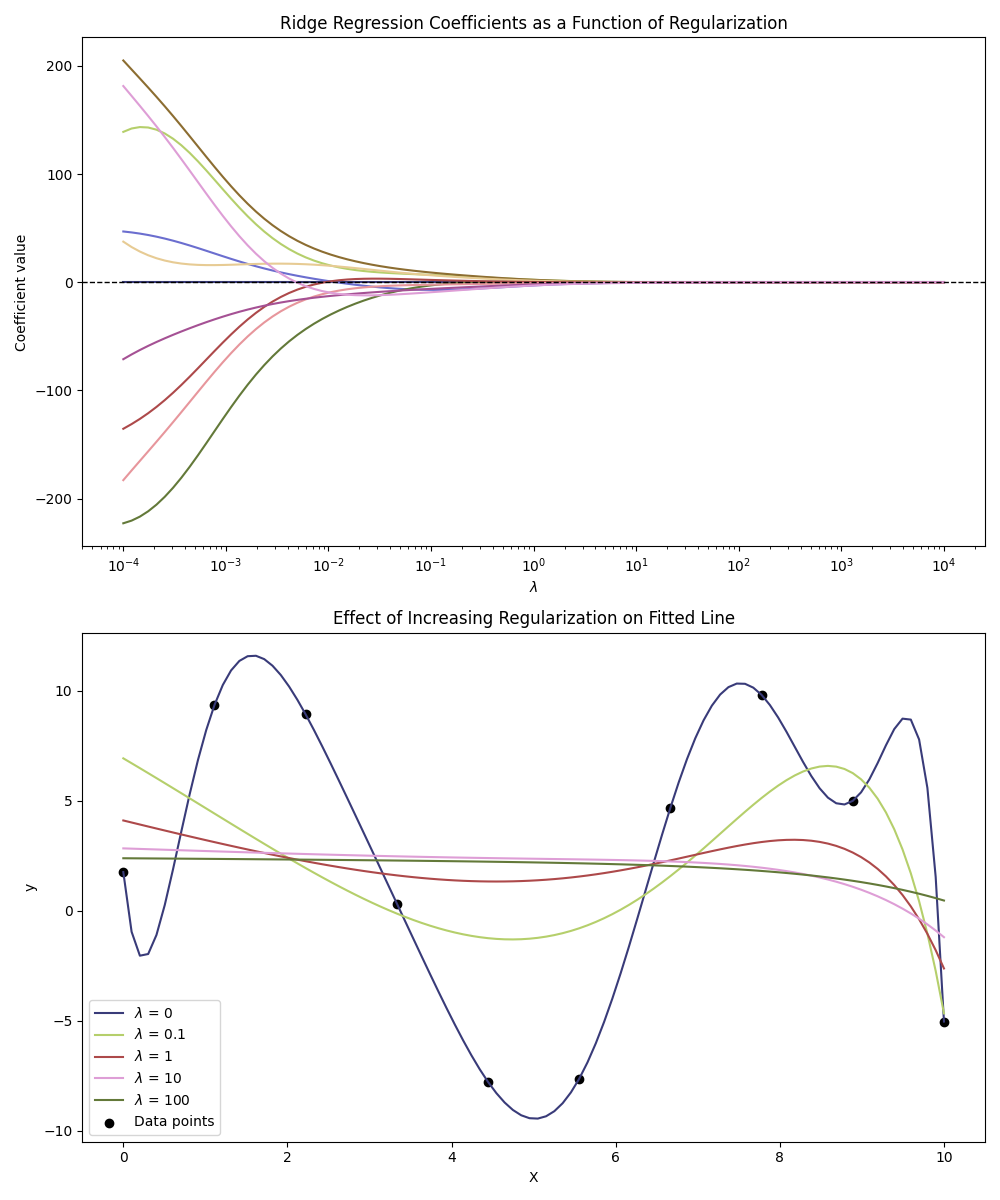
\includegraphics[width=1.0\linewidth]{img/ridge_lambda_effect}
		\caption{Ridge Regression Coefficients and the Effect of Regularization. The \textbf{top plot} shows Ridge Regression coefficients as a function of the regularization parameter $\lambda$. Each line represents a different feature's coefficient, demonstrating how increasing $\lambda$ causes the coefficients to shrink towards zero. The \textbf{bottom plot} illustrates the effect of $\lambda$ on the fitted non-linear model for 10 data points. As $\lambda$ increases, the model transitions from overfitting (high variance) to better generalization (low variance), as seen by the smoothing of the fitted lines.}
		\label{fig:ridgelambdaeffect}
	\end{figure}
	
	
	\subsubsection*{Properties and Benefits}
	\begin{itemize}
		\item \textbf{Bias-Variance Tradeoff}: By introducing the penalty term, Ridge Regression can reduce the variance of the model at the cost of introducing some bias. This tradeoff can lead to better generalization performance compared to OLS, especially when dealing with high-dimensional data \cite{sohilIntroductionStatisticalLearning2022}.
		\item \textbf{Handling Multicollinearity}: Multicollinearity occurs when input features are highly correlated, making it difficult to estimate their individual effects. Ridge Regression mitigates this issue by shrinking the coefficients, thus providing more stable estimates \cite{hoerlRidgeRegressionBiased1970, marquardtRidgeRegressionPractice1975}.
	\end{itemize}
	
	
	
\section*{Methods}

\section*{Results}

\section*{Discussion}

\newpage
\printbibliography

\end{document}